\documentclass[border=10pt]{standalone}
\usepackage{pgfplots}
\pgfplotsset{compat=1.18}
\usepgfplotslibrary{fillbetween}
\begin{document}
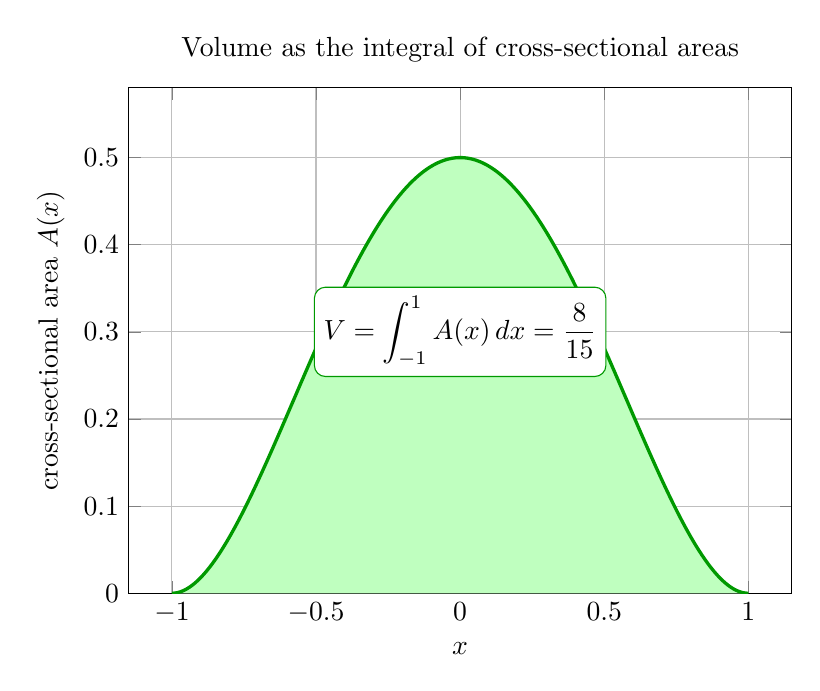
\begin{tikzpicture}
\begin{axis}[
    width=10cm, height=8cm,
    xmin=-1.15, xmax=1.15, ymin=0, ymax=0.58,
    xlabel={$x$}, ylabel={cross-sectional area $A(x)$},
    title={Volume as the integral of cross-sectional areas},
    grid=both, samples=200,
]
\addplot[name path=A, green!60!black, very thick, domain=-1:1] {0.5*(1-x^2)^2};
\addplot[name path=z, draw=none, domain=-1:1] {0};
\addplot[green!25] fill between[of=A and z];
\node[draw=green!60!black, fill=white, rounded corners] at (axis cs:0,0.30)
   {$V=\displaystyle\int_{-1}^{1} A(x)\,dx=\frac{8}{15}$};
\end{axis}
\end{tikzpicture}
\end{document}
